\documentclass[english]{article}
\usepackage[T1]{fontenc}
\usepackage[utf8]{inputenc}
\usepackage[italian]{babel}
\usepackage{graphicx}
\usepackage{subcaption}
\usepackage{caption}
\usepackage{gensymb}
\usepackage{amsmath,bm}
\usepackage{siunitx}
\usepackage{float}
\usepackage{hyperref}
\captionsetup{tableposition=top,figureposition=bottom,font=footnotesize}
\renewcommand{\vec}{\mathbf}
\usepackage{upgreek}
\usepackage[a4paper, total={7in, 8in}]{geometry}
\begin{document}
\title{TITOLO:RELAZIONE DI DATA MINING}
\author{Daniele Maria Di Nosse, Angelo Lasala, Raffaele Paradiso}
\date{21/11/2020\newpage}

\maketitle
\tableofcontents{}

\newpage

\section{Introduzione}
Determinare le possibili relazioni che intercorrono fra caratteristiche dei dipendenti di un'azienda può risultare di grande utilità per predire i possibili scenari lavorativi che posso verificarsi e gestire di conseguenza l'organizzazione del personale in maniera ottimale. Nel presente progetto ci si pone l'obiettivo di valutare tali legami tramite un approccio di data mining. Le informazioni che si sono utilizzate sono relative ad un data frame fittizio (leggermente modificato) generato da IBM e presente sul portale Kaggle(URL \url{https://www.kaggle.com/pavansubhasht/ibm-hr-analytics-attrition-dataset}). Non ci si è posto un obiettivo principale, ovvero la determinazione di legami, correlazioni e classificazioni relativi ad un singolo attributo rispetto a tutti gli altri, ma si è proceduto in maniera più generale ricoprendo uno spettro più ampio di possibili relazioni fra tutte le variabili.

Sebbene i dati a disposizione siano stati divisi in due sotto insiemi, uno di Train ed uno di Test, si è deciso di utilizzare l'intero insieme di records per tutti i tasks che non concernono algoritmi di Machine Learning
\section{Data Understanding}
\subsection{Data Semantics}
Nella prima fase dell'elaborazione si è studiato il data frame nella sua forma originale (Train $+$ Test), valutando il numero degli attributi, la loro natura e dominio. 

\begin{figure}[H]
\centering
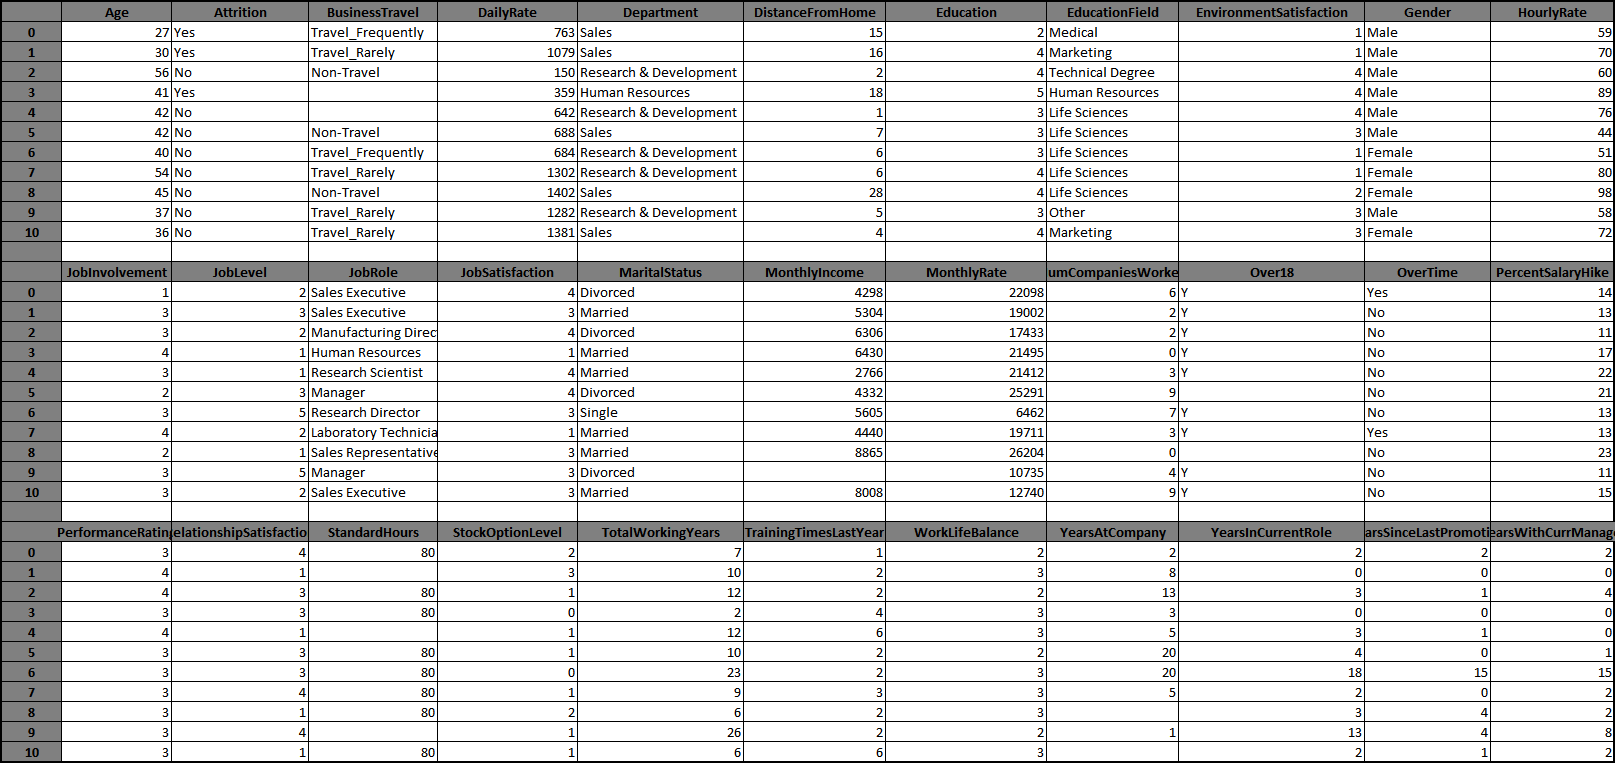
\includegraphics[scale=0.55]{DFhead(10).png}
\caption{Primi 10 valori di tutti gli attributi}
\end{figure}

Come si può notare dalla tabella precedente, il numero di attributi è pari a 33. Si dividono in attributi numerici e categorici, ma ad uno sguardo più attento si nota che alcuni di essi, come, ad esempio, Education o Enviroment Satisfaction, presentano valori numerici che poco si adattano al loro significato. Si ha infatti che sussistono le seguenti uguaglianze 

Education

1 : 'Below College'

2 : 'College'

3 : 'Bachelor'

4 : 'Master'

5 : 'Doctor'


EnvironmentSatisfaction

1 : 'Low'

2 : 'Medium'

3 : 'High'

4 : 'Very High'


JobInvolvement

1 : 'Low'

2 : 'Medium'

3 : 'High'

4 : 'Very High'

JobSatisfaction

1 : 'Low'

2 : 'Medium'

3 : 'High'

4 : 'Very High'


PerformanceRating

1 : 'Low'

2 : 'Good'

3 : 'Excellent'

4 : 'Outstanding'


RelationshipSatisfaction

1 : 'Low'

2 : 'Medium'

3 : 'High'

4 : 'Very High'


WorkLifeBalance

1 : 'Bad'

2 : 'Good'

3 : 'Better'

4 : 'Best'
\\ Di conseguenza, il dominio di tali attributi è di tipo categorico od ordinale e non numerico. Organizzando tutte le variabili per la loro tipologia, si ottiene che
\begin{figure}[h]
\centering
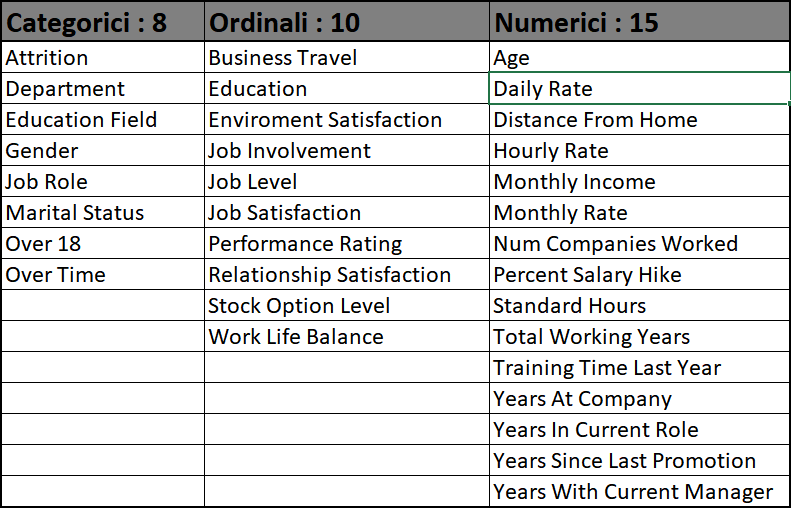
\includegraphics[scale=0.55]{semantics.png}
\caption{Classificazione degli attributi}
\end{figure}

Per quanto riguarda il range di valori degli attributi risulta essere, come è possibile aspettarsi da quanto detto, molto più discretizzato per gli attributi ordinali che per gli attributi numerici. Inoltre, differisce molto da attributo ad attributo (anche di 4 ordini di grandezza), cosa che sottolinea sin da questo punto l'importanza di una trasformazione delle variabili.

\begin{figure} [h]
\centering
\begin{subfigure}{.5\textwidth}
\centering
  \includegraphics[width=.5\linewidth]{age.png}
  \caption{Age}
  \label{fig:sfig1}
\end{subfigure}%
\begin{subfigure}{.5\textwidth}
\centering
  \includegraphics[width=.5\linewidth]{dailyrate.png}
  \caption{Daily Rate}
  \label{fig:sfig2}
\end{subfigure}%
\begin{subfigure}{.5\textwidth}
  \centering
  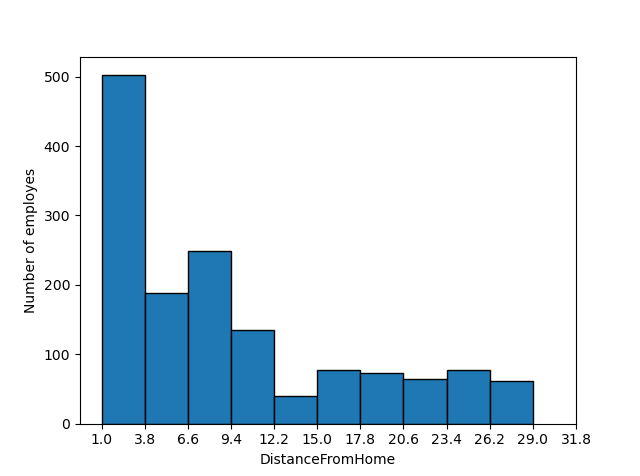
\includegraphics[width=.5\linewidth]{DistanceFromHome.png}
  \caption{DistanceFromHome}
  \label{fig:sfig3}
\end{subfigure}
\begin{subfigure}{.5\textwidth}
  \centering
  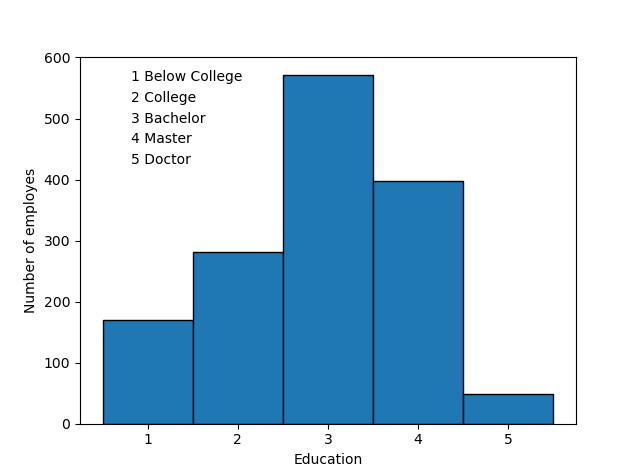
\includegraphics[width=.5\linewidth]{Education.png}
  \caption{Education}
  \label{fig:sfig4}
\end{subfigure}%
\begin{subfigure}{.5\textwidth}
  \centering
  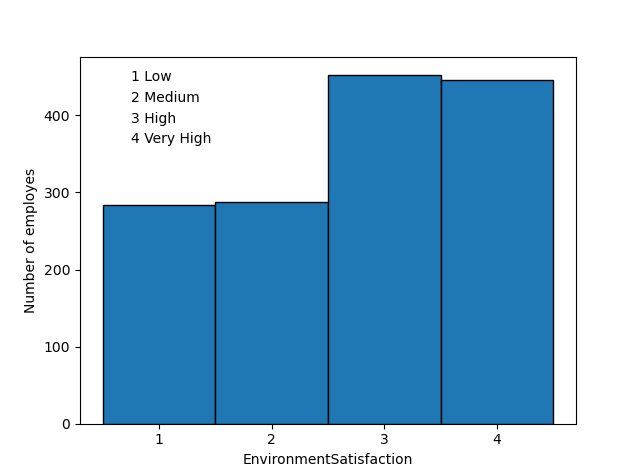
\includegraphics[width=.5\linewidth]{Enviroment Satisfaction.png}
  \caption{Enviroment Satisfaction}
  \label{fig:sfig5}
\end{subfigure}%
\begin{subfigure}{.5\textwidth}
  \centering
  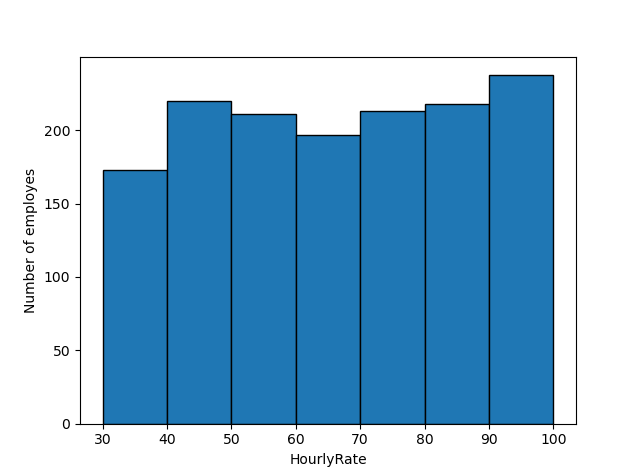
\includegraphics[width=.5\linewidth]{HourlyRate.png}
  \caption{Hourly Rate}
  \label{fig:sfig6}
\end{subfigure}
\begin{subfigure}{.5\textwidth}
  \centering
  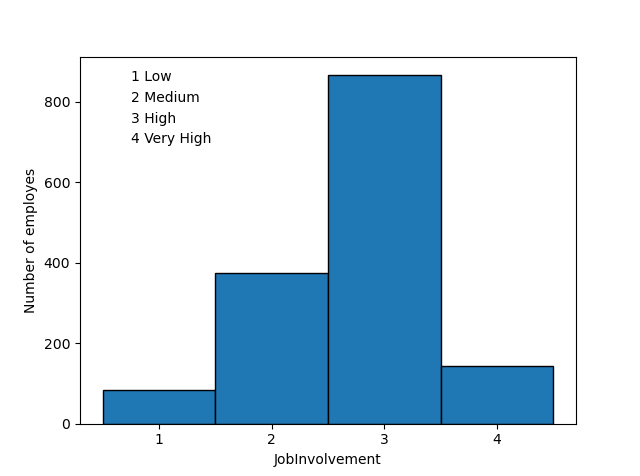
\includegraphics[width=.5\linewidth]{JobInvolvement.png}
  \caption{Job Involvement}
  \label{fig:sfig7}
\end{subfigure}%
\begin{subfigure}{.5\textwidth}
  \centering
  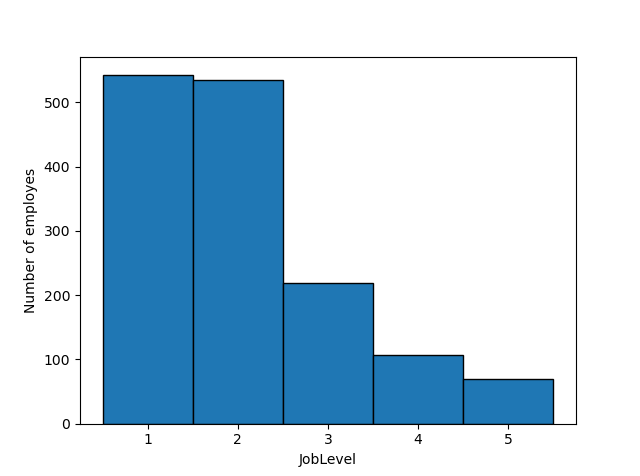
\includegraphics[width=.5\linewidth]{joblevel.png}
  \caption{Job Level}
  \label{fig:sfig8}
\end{subfigure}
\end{figure}

\newpage
\begin{figure} [h]
\centering
\begin{subfigure}{.5\textwidth}
  \centering
  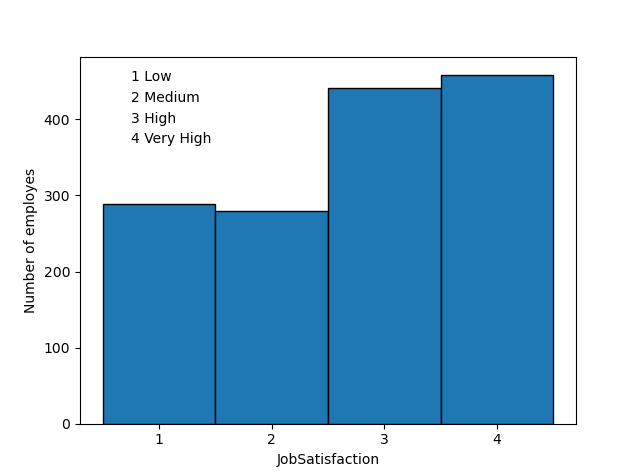
\includegraphics[width=.8\linewidth]{JobSatisfaction.png}
  \caption{Job Satisfaction}
  \label{fig:sfig9}
\end{subfigure}%
\begin{subfigure}{.5\textwidth}
  \centering
  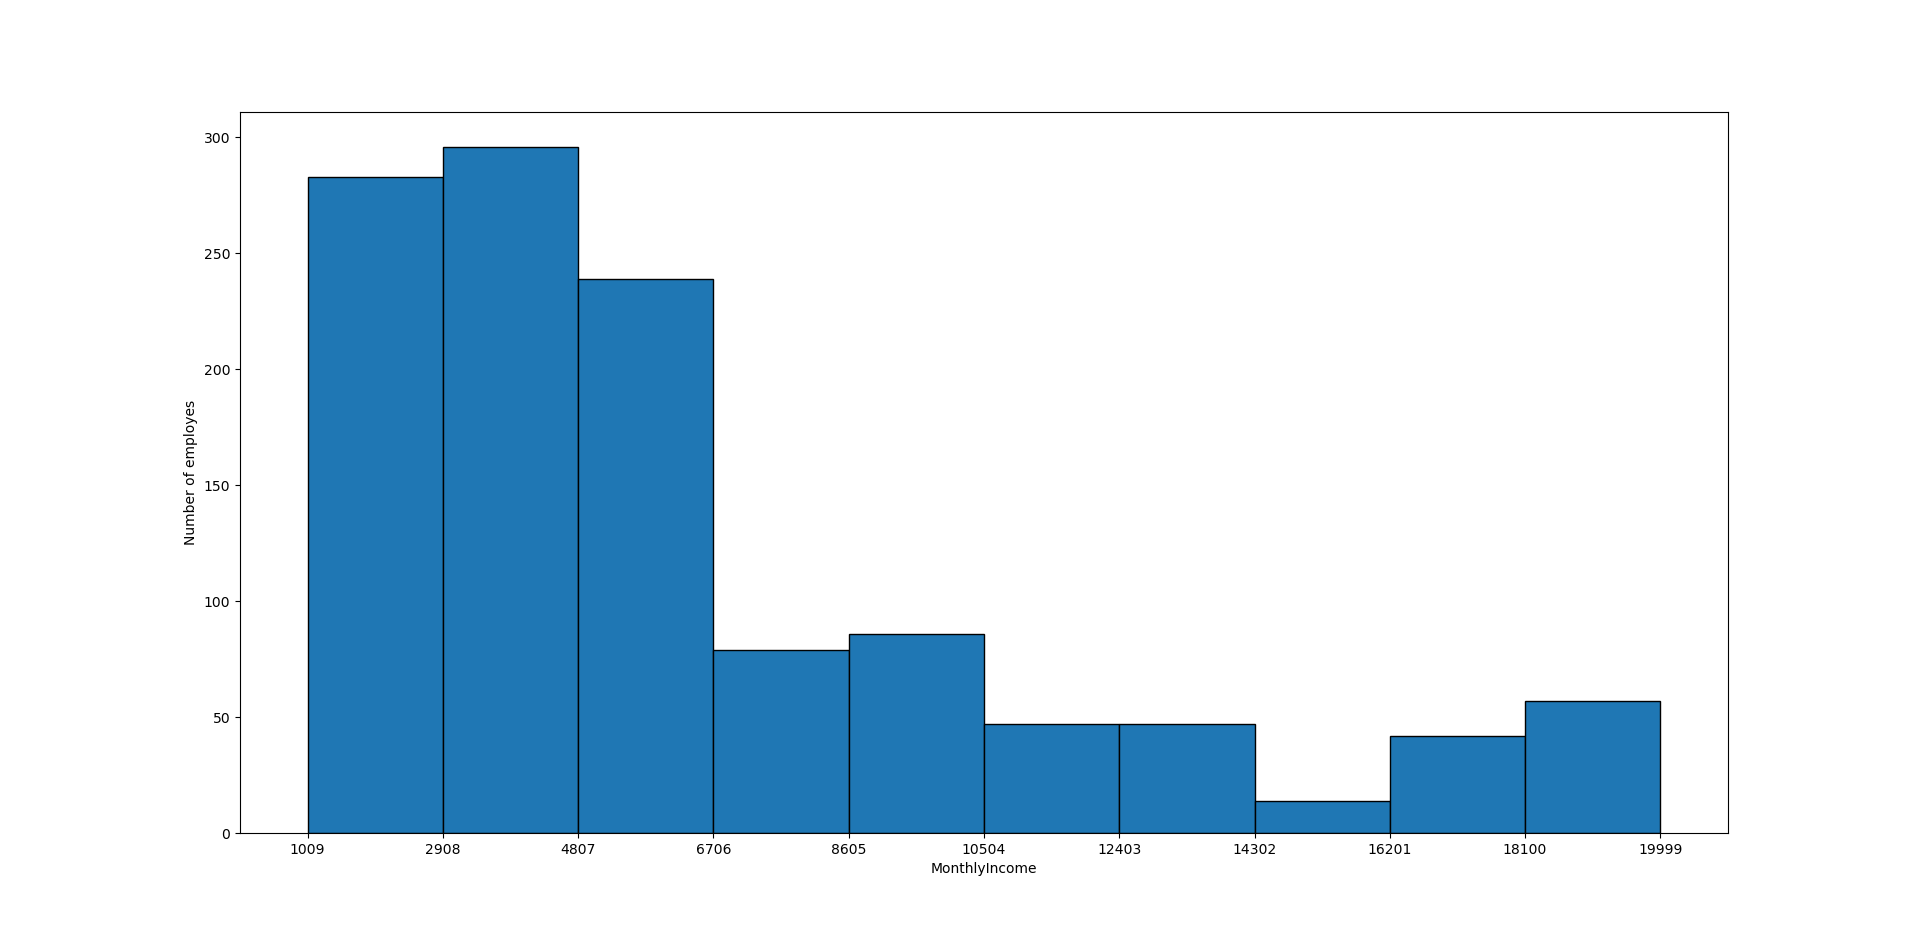
\includegraphics[width=.8\linewidth]{MonthlyIncome.png}
  \caption{Montlhy Income}
  \label{fig:sfig10}
\end{subfigure}
\begin{subfigure}{.5\textwidth}
  \centering
  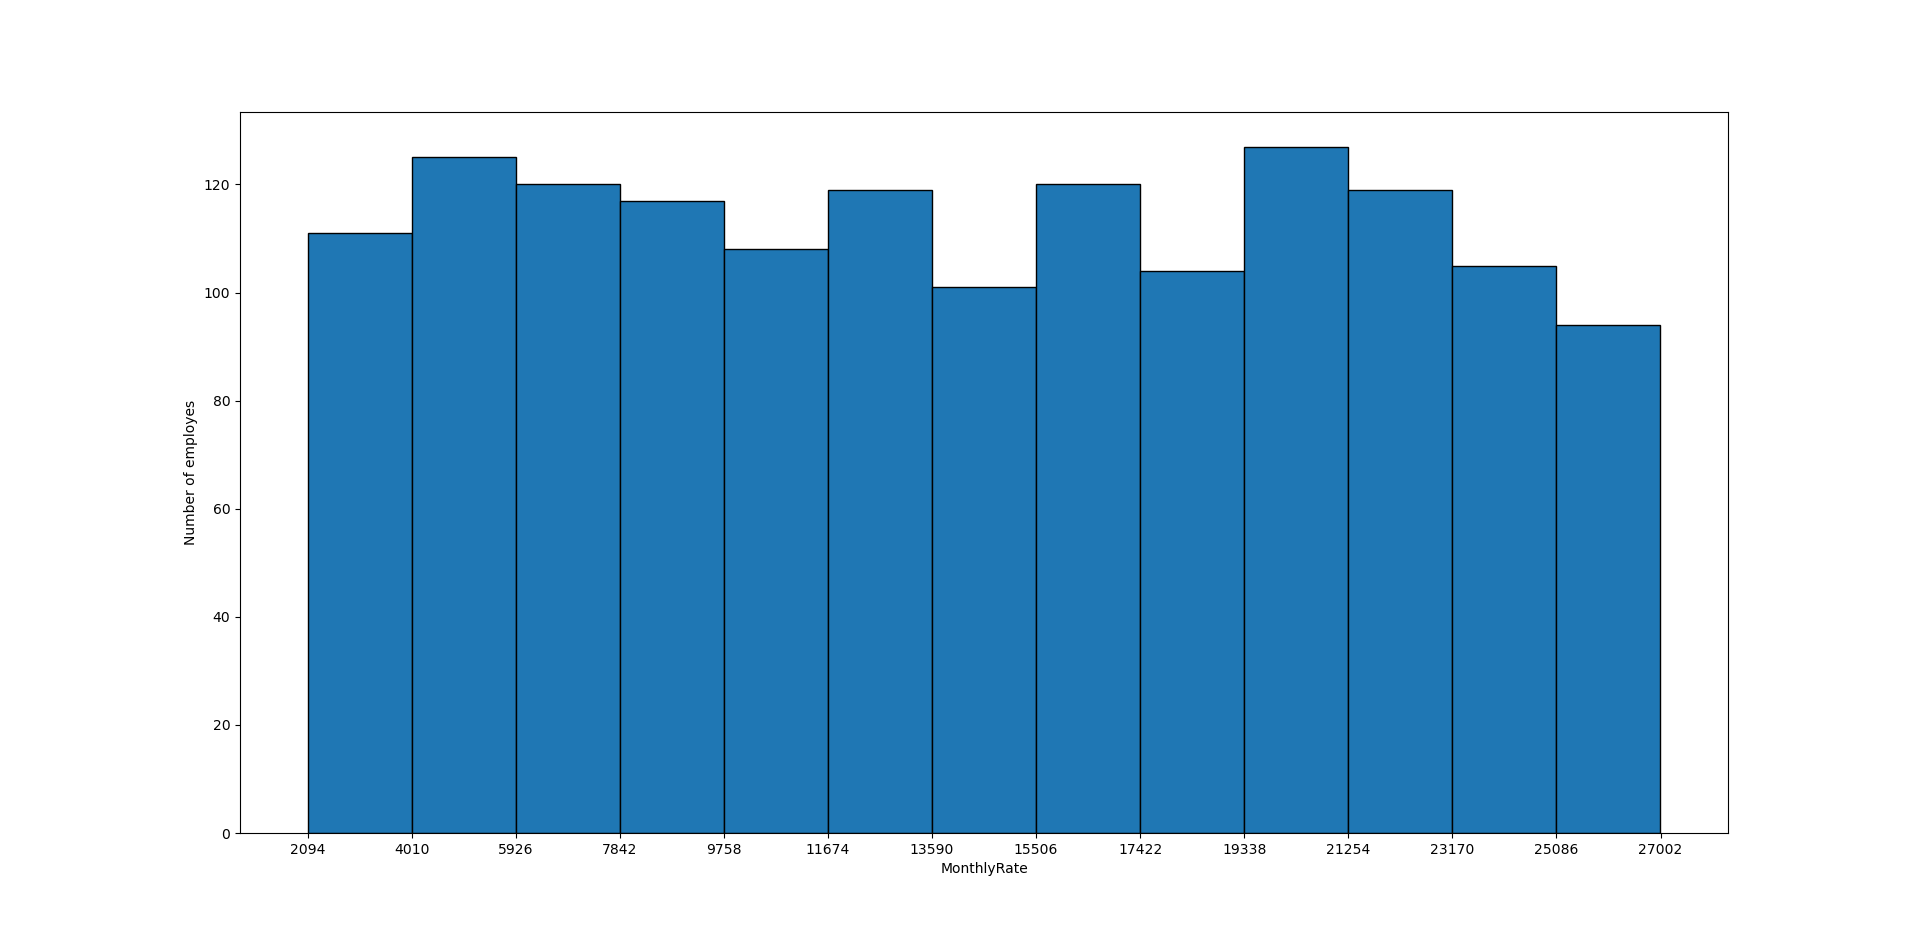
\includegraphics[width=.8\linewidth]{MonthlyRate.png}
  \caption{MonthlyRate}
  \label{fig:sfig11}
\end{subfigure}%
\begin{subfigure}{.5\textwidth}
  \centering
  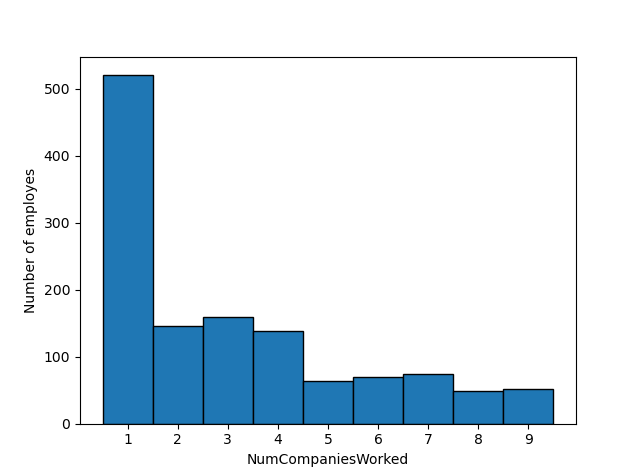
\includegraphics[width=.8\linewidth]{numcompanieswork.png}
  \caption{Num Companies Worked}
  \label{fig:sfig12}
\end{subfigure}
\begin{subfigure}{.5\textwidth}
  \centering
  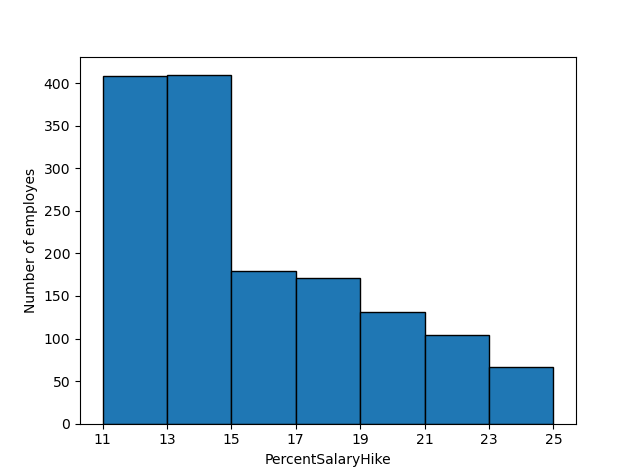
\includegraphics[width=.8\linewidth]{PercentSalaryHike.png}
  \caption{Percent Salary Hike}
  \label{fig:sfig13}
\end{subfigure}%
\begin{subfigure}{.5\textwidth}
  \centering
  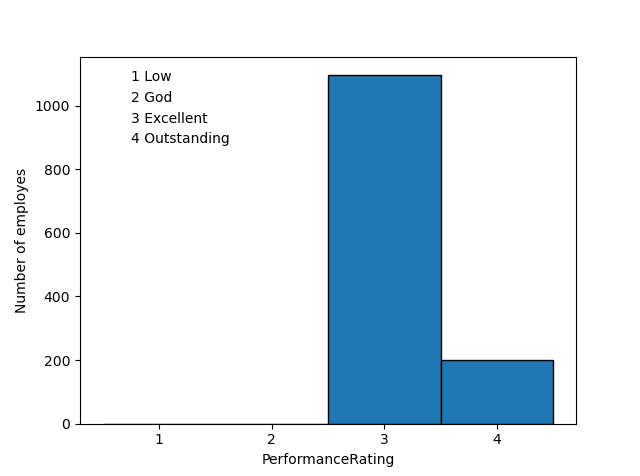
\includegraphics[width=.8\linewidth]{Performance Rating.png}
  \caption{Performance Rating}
  \label{fig:sfig14}
\end{subfigure}
\begin{subfigure}{.5\textwidth}
  \centering
  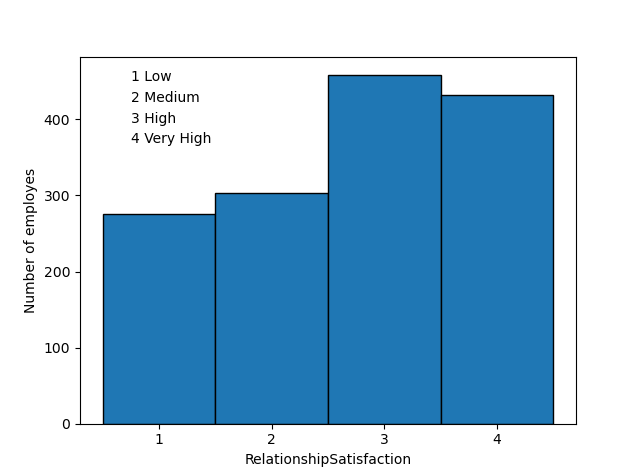
\includegraphics[width=.8\linewidth]{Relationship Satisfaction.png}
  \caption{Relationship Satisfaction}
  \label{fig:sfig15}
\end{subfigure}%
\begin{subfigure}{.5\textwidth}
  \centering
  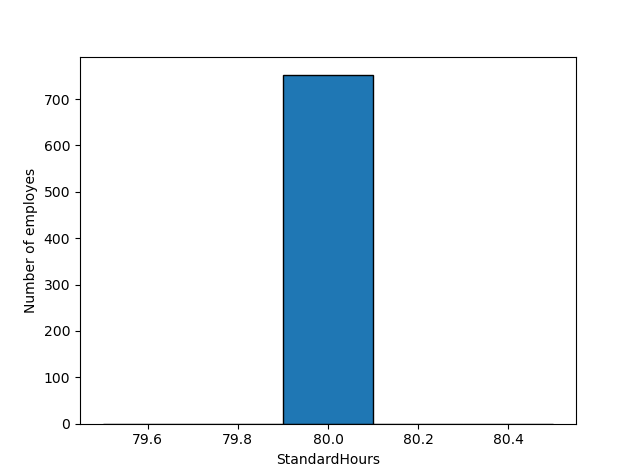
\includegraphics[width=.8\linewidth]{Standard Hours.png}
  \caption{Standard Hours}
  \label{fig:sfig16}
\end{subfigure}
\end{figure}

\newpage
\begin{figure} [h]
\centering
\begin{subfigure}{.5\textwidth}
  \centering
  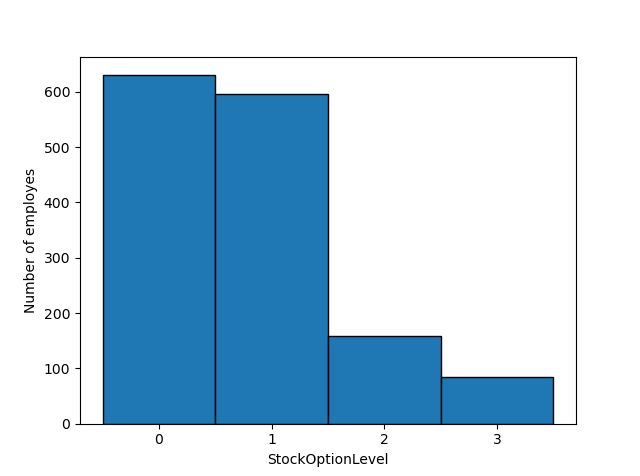
\includegraphics[width=.8\linewidth]{Stock Option Level.png}
  \caption{Stock Option Level}
  \label{fig:sfig17}
\end{subfigure}%
\begin{subfigure}{.5\textwidth}
  \centering
  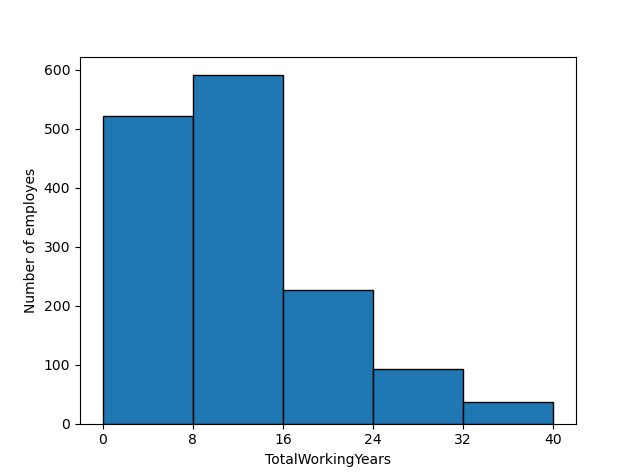
\includegraphics[width=.8\linewidth]{Total Working Years.png}
  \caption{Total Working Years}
  \label{fig:sfig18}
\end{subfigure}
\begin{subfigure}{.5\textwidth}
  \centering
  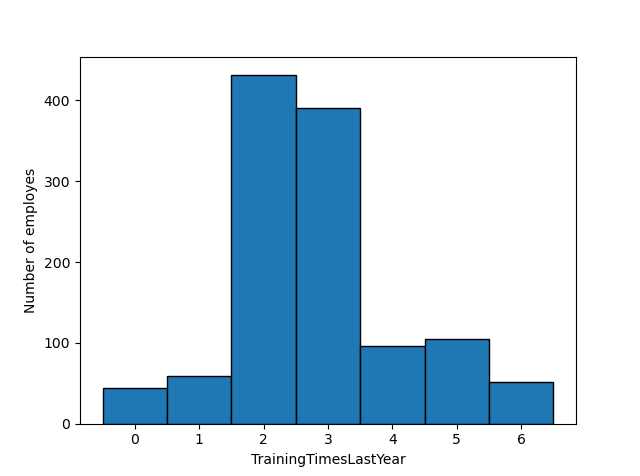
\includegraphics[width=.8\linewidth]{Training Time Last Year.png}
  \caption{Training Time Last Year}
  \label{fig:sfig19}
\end{subfigure}%
\begin{subfigure}{.5\textwidth}
  \centering
  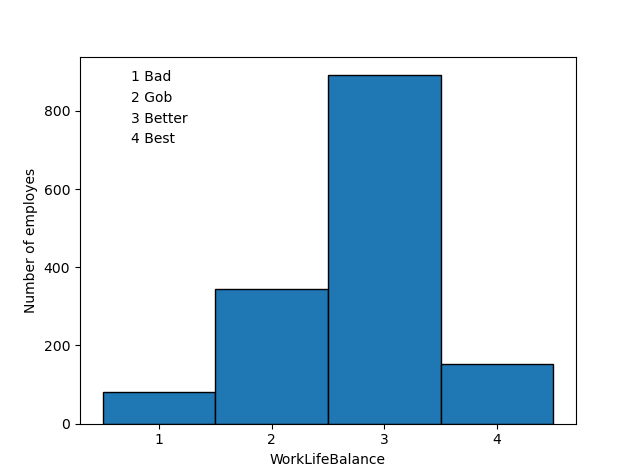
\includegraphics[width=.8\linewidth]{Work Life Balance.png}
  \caption{Work Life Balance}
  \label{fig:sfig20}
\end{subfigure}
\begin{subfigure}{.5\textwidth}
  \centering
  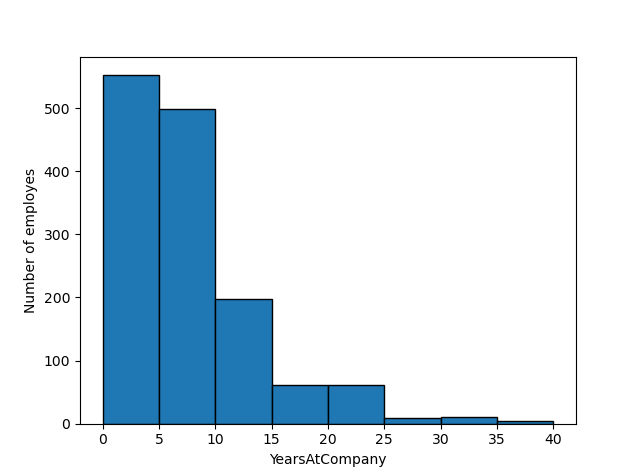
\includegraphics[width=.8\linewidth]{YearsAtCompany.png}
  \caption{Years At Company}
  \label{fig:sfig21}
\end{subfigure}%
\begin{subfigure}{.5\textwidth}
  \centering
  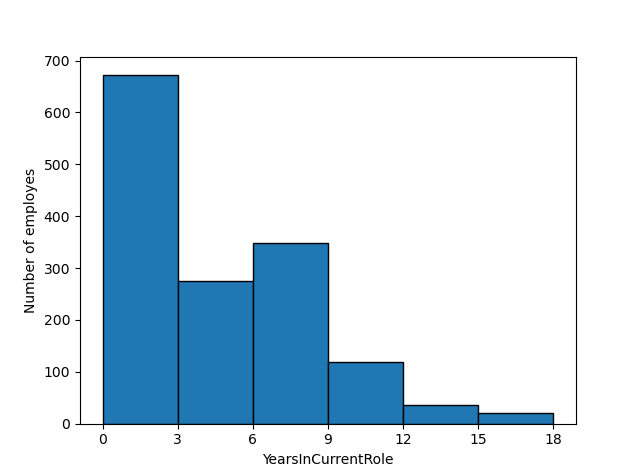
\includegraphics[width=.8\linewidth]{YearsInCurrentRole.png}
  \caption{Years In Current Role}
  \label{fig:sfig22}
\end{subfigure}
\begin{subfigure}{.5\textwidth}
  \centering
  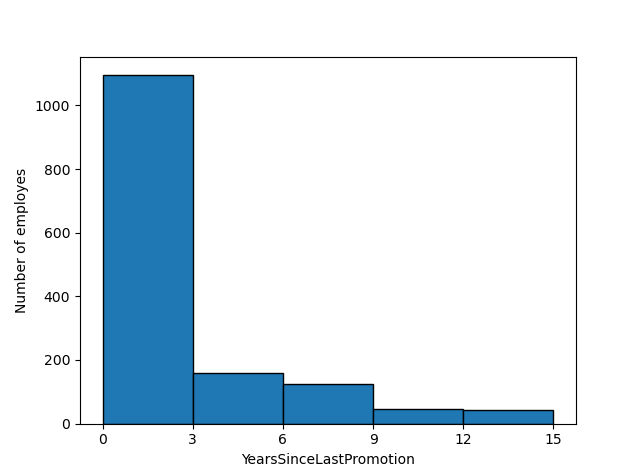
\includegraphics[width=.8\linewidth]{YearsSinceLastPromotion.png}
  \caption{Years Since Last Promotion}
  \label{fig:sfig23}
\end{subfigure}%
\begin{subfigure}{.5\textwidth}
  \centering
  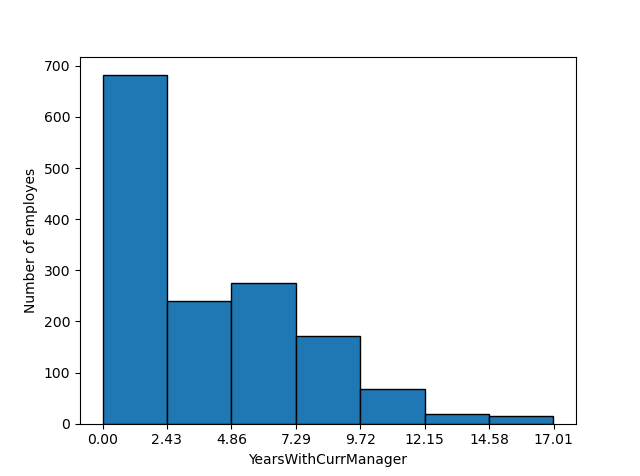
\includegraphics[width=.8\linewidth]{YearsWithCurrManager.png}
  \caption{Years With Current Manager}
  \label{fig:sfig24}
\end{subfigure}
\end{figure}

\section{Clustering}

\section{Conclusioni}
\end{document}
